% Header
\documentclass[12pt,a4paper]{report}
\usepackage[utf8x]{inputenc}
\usepackage[T1]{fontenc}
\usepackage{geometry}
\usepackage{graphicx}
\usepackage[danish]{isodate}
\usepackage[danish]{babel}
\usepackage{url}
\usepackage{color}
\usepackage{ulem}
\usepackage{titlesec}
\usepackage{hyperref}
\usepackage{float}
\usepackage{tabularx}
\usepackage{ucs}

% lstlisting to show code nicely
\usepackage{listings}

\definecolor{mygreen}{rgb}{0,0.6,0}
\definecolor{mygray}{rgb}{0.5,0.5,0.5}
\definecolor{mymauve}{rgb}{0.58,0,0.82}

\lstset{
  backgroundcolor=\color{white},   % choose the background color; you 
  %basicstyle=\footnotesize,
  basicstyle=\ttfamily,            % the size of the fonts that are used 
  breakatwhitespace=false,         % sets if automatic breaks should 
  breaklines=true,                 % sets automatic line breaking
  captionpos=b,                    % sets the caption-position to bottom
  commentstyle=\color{mygreen},    % comment style
  deletekeywords={...},            % if you want to delete keywords from 
  escapeinside={\%*}{*)},          % if you want to add LaTeX within 
  inputencoding=utf8x,
  extendedchars=true,              % lets you use non-ASCII characters; 
  frame=single,                    % adds a frame around the code
  keepspaces=true,                 % keeps spaces in text, useful for 
  keywordstyle=\color{blue},       % keyword style
  language={[Sharp]C},             % the language of the code
  morekeywords={*,...},            % if you want to add more keywords to 
  numbers=left,                    % where to put the line-numbers; 
  numbersep=5pt,                   % how far the line-numbers are from 
  numberstyle=\tiny\color{mygray}, % the style that is used for the 
  rulecolor=\color{black},         % if not set, the frame-color may be 
  showspaces=false,                % show spaces everywhere adding 
  showstringspaces=false,          % underline spaces within strings 
  showtabs=false,                  % show tabs within strings adding 
  stepnumber=2,                    % the step between two line-numbers. 
  stringstyle=\color{mymauve},     % string literal style
  tabsize=2,                       % sets default tabsize to 2 spaces
  title=\lstname,                  % show the filename of files included 
  literate={æ}{{\ae}}1
           {ø}{{\o}}1
           {å}{{\aa}}1
           {Æ}{{\AE}}1
           {Ø}{{\O}}1
           {Å}{{\AA}}1
}



% Fonts
\usepackage{helvet} % <-- Helvetica (sans)
\usepackage[sc]{mathpazo} % <-- Palatino (serif)
\linespread{1.05}   % Extra linespread for Palatino

% Extra settings
% \setlength\parindent{0pt} % For at fjerne automatiske indrykninger
% \let\clearpage\relax % For at fjerne alle clearpage sideskift

% Meta (til titelblad)
% HUSK; at rette Jonas i titelbladet.
\newcommand{\rtitle}{Elektroniske lommepenge} %<----
\newcommand{\rtheme}{Programmering og problemløsning}
\newcommand{\rperiod}{P2, 2013}
\newcommand{\rdeadline}{22. maj 2013} %<----Erstattes med rapportens deadline
\newcommand{\rprints}{10} %<---- Erstattes med oplægsantal
\newcommand{\rappendices}{1 (måske)} %<---- Erstattes med bilagsantal og art
\newcommand{\rlastpage}{ca 50-60 stykker} %<---- Erstattes med sideantal

%\newcommand{\code}[1]{\lstinline!#1!}
\newcommand{\code}[1]{\lstinline{#1}} %<---- Er fikset, skriver nu i mono :). (Skulle gerne skrive tekst i mono, til klasse navne. Ser ikke ud til at virke)

%%Jonas
\usepackage{lastpage}

%relinput
\usepackage{xstring}
\usepackage{etoolbox}

%Init a new array
% #1 = array name
\newcommand\arrayinit[1]{%
	\newcounter{#1-cnt}%
}

%set a value in an array
% #1 = array name
% #2 = array index
% #3 = new value
\newcommand\arraysetvalue[3]{%
	\cslet{#1-#2}{#3}%
}

%append new value to the end af array - push
% #1 = array name
% #2 = append value
\newcommand\arraypush[2]{%
	\stepcounter{#1-cnt}%
	\arraysetvalue{#1}{\arabic{#1-cnt}}{#2}
}

%Get value at position
% #1 = array name
% #2 = array index
% NB: To use counters, do: \arraygetvalue{ARR}{\arabic{COUNTER}}
\newcommand\arraygetvalue[2]{%
	\csuse{#1-#2}%
}

%Delete value at position
% #1 = array name
% #2 = array index
\newcommand\arraydeletevalue[2]{%
	\csundef{#1-#2}%
}

%Delete the last index
% #1 = array name
\newcommand\arraydeletelast[1]{%
	\arraydeletevalue{#1}{\arabic{#1-cnt}}%
	\addtocounter{#1-cnt}{-1}%
}

%Get last value in array and delete the last index; pop
% #1 = array name
\newcommand\arraypop[1]{%
	\arraygetvalue{#1}{\arabic{#1-cnt}}%
	\arraydeletelast{#1}%
}

%\newcounter{tempcount} % for temporary usage

\newcommand\arrayloop[1]{%
\setcounter{tempcount}{0}%
	Looping \arabic{tempcount} to \arabic{#1-cnt}%
	
	\loop\ifnum\value{tempcount}<\value{#1-cnt}%
		\stepcounter{tempcount}%
		\arraygetvalue{#1}{\arabic{tempcount}} \\ %
	\repeat%
}
 %Enable this for debug..
\arrayinit{relinputlayerfilepaths}


\newcommand\lastsubstrposition{}
\newcommand\lastindex[2]{%
	\StrCount{#1}{#2}[\numberofsubstr]%
	\StrPosition[\numberofsubstr]{#1}{#2}[\lastsubstrposition]%
}


\newcommand\relinputfilepath{}
\newcommand\relinputfilename{}
\newcommand\relinputtempstrlen{}
\newcommand\relinputparseinput[1]{%
	%get the pos of the last slash
	\lastindex{#1}{/}%
	
	%Whatever's left of the last slash is the path
	\StrLeft{#1}{\lastsubstrposition}[\relinputfilepath]%
	
	%Whatever's right of the last slash is the filename
	\StrLen{#1}[\relinputtempstrlen]%
	\StrRight{#1}{\the\numexpr\relinputtempstrlen-\lastsubstrposition}[\relinputfilename]%
}


\newcommand\filetoinclude{}
\newcommand\relinput[1]{
	%Parse the input
	\relinputparseinput{#1}%
	
	%Push the path to the array
	\arraypush{relinputlayerfilepaths}{\relinputfilepath}%
	
	%Create the total path to the file to be included
	\relinputinputconcatpath{relinputlayerfilepaths}{\relinputfilename}%
	\renewcommand\filetoinclude{\completepath}%
	\input{\filetoinclude}%
	
	%Delete the last index in the array
	\arraydeletelast{relinputlayerfilepaths}%
}


\global\def\completepath{}
\newcounter{concatpathcounter}
\newcommand\relinputinputconcatpath[2]{
	\global\edef\completepath{}%
	\setcounter{concatpathcounter}{0}%
	\loop\ifnum\value{concatpathcounter}<\value{#1-cnt}%
		\stepcounter{concatpathcounter}%
		\global\edef\completepath{\completepath\arraygetvalue{#1}{\arabic{concatpathcounter}}}%
	\repeat%
	\global\edef\completepath{\completepath#2}%
}


%Forside stuff
\definecolor{Sapphire}{RGB}{28,117,188}
\usepackage[x11names,rgb,usenames,dvipsnames,svgnames,table]{xcolor}


% Document root
\begin{document}

%Forside + random hacks for isolated env
\begin{titlepage}
\newcommand{\HRule}[1]{\hfill \rule{0.2\linewidth}{#1}}

\definecolor{grey}{rgb}{0.9,0.9,0.9}
\newgeometry{top=1.5in,bottom=1in,right=0cm,left=0cm}
\thispagestyle{empty}
\centering {\LARGE Aalborg Universitet}
\vspace*{1.5cm}

\noindent \colorbox{Sapphire}{
\parbox[t]{1.0\linewidth}{
\centering \fontsize{50pt}{80pt}\selectfont
\vspace*{1.0cm}
        \textcolor{White}{
        \sffamily{
Elektroniske Lommepenge \\[3pt]
        %\LARGE Elektroniske Lommepenge \\
        }
\vspace*{0.7cm}
        }
}
}
\\[2em]
\huge P2-Projekt

\vfill
\flushright
\flushright \rule[20pt]{0.1pt}{9em} \begin{minipage}[b]{0.50\linewidth}
{
\Large
\textbf{Gruppe A325:} \\
Anders Trier Olesen\\
Frederik Meyer Bønneland\\
Jannek Alexander Westerhof Bossen\\
Jonas Christoffersen\\
Katrine Sofie Tjell\\
Kevin Brämer\\
Ólavur Debes Joensen\\
}
\end{minipage}
\clearpage 
\thispagestyle{empty}
\end{titlepage}
\newpage
\thispagestyle{empty}
\mbox{}
% AAU Titelblad
% Muligt at indsætte denne i PDF'ens indholdsfortegnelse?
\begin{titlepage}
\newgeometry{top=1in,bottom=1in,right=1in,left=1in}
\small
\begin{nopagebreak}
{\samepage 
\begin{tabular}{r}
\parbox{\textwidth}{  \raisebox{11mm}{
\includegraphics[height=1.2cm]{Billeder/aau-logo.pdf}}
\hfill \begin{tabular}{l}
{\sf\small \textbf{Det Teknisk-Naturvidenskabelige Basis{\aa}r }}\\
{\sf\small  \textbf{Datalogi og Software}} \\
{\sf\small Strandvejen 12-14} \\
{\sf\small Telefon 96 35 97 31} \\
{\sf\small Fax 98 13 63 93} \\
{\sf\small http://tnb.aau.dk}
\end{tabular}}
\\
\end{tabular}

\begin{tabular}{cc}
\parbox{7cm}{
\begin{description}

\item {\bf Titel:} 

\rtitle
  
\item {\bf Tema:} 

\rtheme

\end{description}

\parbox{8cm}{

\begin{description}
\item {\bf Projektperiode:}\\
   \rperiod \\
  \hspace{4cm}
\item {\bf Projektgruppe:}\\
  B228\\
  \hspace{4cm}
\item {\bf Deltagere:}\\
Bossen, Jannek Alexander Westerhof\\
Brämer, Kevin\\
Bønneland, Frederik Meyer\\
Joensen, Ólavur Debes\\
Olesen, Anders Trier\\
Tjell, Katrine Sofie\\
  \hspace{2cm}
\item {\bf Vejledere:}\\
 Michael Skøtt Madsen \\
  Amanda Hill \\
\end{description}
}
\begin{description}
\item {\bf Oplagstal:} 10
\item {\bf Sidetal:} 
\item {\bf Bilagsantal og --art:} 6 
\item {\bf Afsluttet den} \rdeadline
\end{description}
\vfill } &
\parbox{7cm}{
  \vspace{.15cm}
  \hfill 
  \begin{tabular}{l}
  {\bf Synopsis:}\bigskip \\
  \fbox{
    \parbox{6.5cm}{\bigskip
     {\vfill{\small Dette projekt handler om komprimering af SMS-beskeder. Problemstilling i projeket er, at en SMS-besked har en begrænsning på 160 tegn og hvis denne begrænsning overskrides betales der SMS-takst for hver påbegyndt besked. I rapporten undersøges hvilke løsninger der allerede findes og det diskuteres hvem der kunne være interesseret i en løsning på problemet. Udover rapporten er der udarbejdet et program som kan komprimere og dekomprimere en tekstbesked, hvorved det bliver muligt at sende flere tegn i samme SMS. Herved kan vi konkludere at det er muligt at sparer brugeren for dobbelt SMS-takst ved at komprimere SMS-beskeder inden afsendelse.
     \bigskip}}
     }}
   \end{tabular}}
\end{tabular}}
\\ \\
\noindent{\footnotesize\emph{Rapportens indhold er frit tilgængeligt, men offentliggørelse (med kildeangivelse) må kun ske efter aftale med forfatterne.}}
\end{nopagebreak}
\end{titlepage}

\newpage
\thispagestyle{empty}
\mbox{}

\addtocontents{toc}{\protect\enlargethispage{-35mm}} %lav en margin i bunden af den forste side af TOC
\addtocontents{toc}{\protect\thispagestyle{empty}} % fjern fra første side af TOC
\tableofcontents
\thispagestyle{empty} %fjern sidetal for den anden side af TOC

%Indledning
\relinput{Indhold/Indledning/indledning}

%ProblemAnalyse
\relinput{Indhold/ProblemAnalyse/ProblemAnalyse}

%Projektafgrænsning
\relinput{Indhold/ProjektAfgransning/ProjektAfgransning}

\newpage
%\thispagestyle{empty} % ved ikke om sidetal skal fjernes fra denne tomme
\mbox{}

%Design Kapitel
\relinput{Indhold/Design/Design}

%Program Kapitel
\relinput{Indhold/Program/Program}

%Konklusions Kapitel
\relinput{Indhold/Konklusion/Konklusion}


% Kilder
\bibliographystyle{plain}
\bibliography{Referencer}

\newgeometry{top=1in,bottom=1in,right=1in,left=1in}
\pagestyle{empty} % Fjerner sidetal fra bilag
\chapter*{Bilag 1: Danske Bank forside}
\setcounter{page}{1}
\thispagestyle{empty} % Fjerner sidetal fra bilag
\begin{figure}[H]
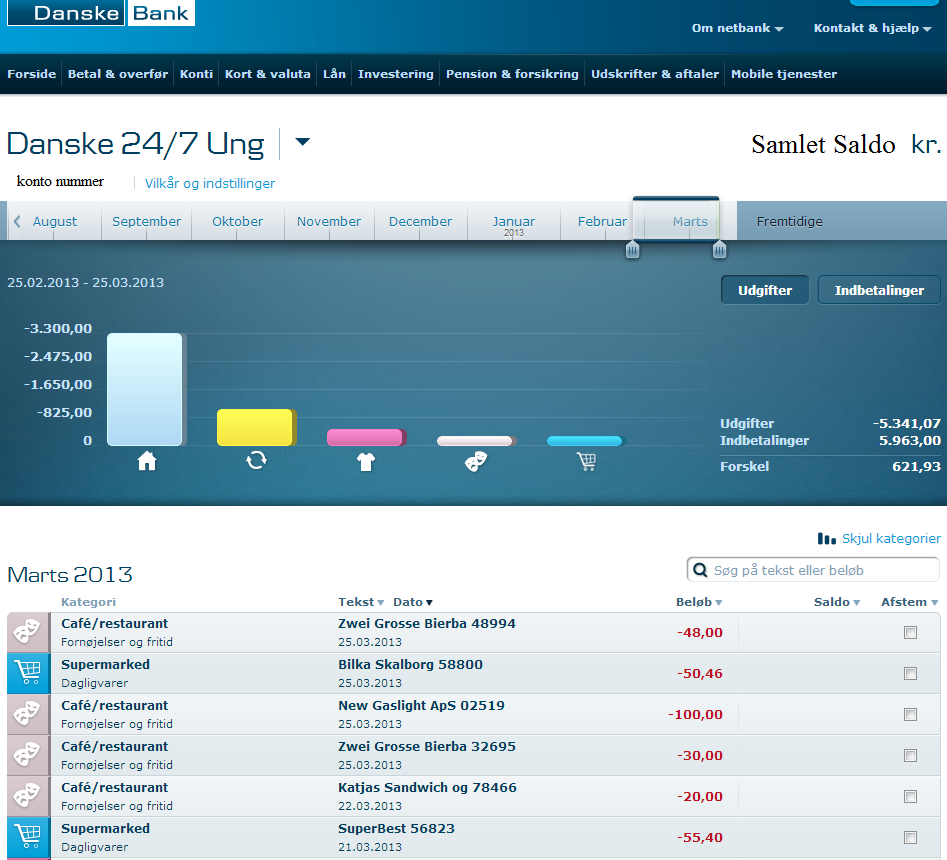
\includegraphics [width=\linewidth]{Billeder/bilagdb1.png}
\caption {Her ses et eksempel på den skærm man bliver mødt af når man logger ind på Danske Banks netbank}
\label {bilagdb1}
\end{figure}

\chapter*{Bilag 2: Databaseforbindelser}
\setcounter{page}{1}
\thispagestyle{empty} % Fjerner sidetal fra bilag
\begin{lstlisting}[caption={Statisk klasse, der forbinder til objekt databasen NDatabase},label={lst:db}]
public static class db
{
	//En string dbFileName med filnavnet på databasen laves
	private const string dbFileName = "database.db";
	
	//Herefter åbnes database forbindelsen
	private static NDatabase.Api.IOdb odb = OdbFactory.Open(dbFileName);

	public static void Store(Transfer transfer)
	{
		//Objektet bliver sendt til databasen
		odb.Store(transfer);
		
		//Databasen bliver tvunget til at opdatere
		odb.Commit();
	}
	
	public static Collection<Transfer> GetTransfersForChild(Child child)
	{
		//Lav en LINQ forespørgsel
		var transfers = from transfer in odb.QueryAndExecute<Transfer>()
						where transfer.Recipient != null && transfer.Recipient.FullName == child.FullName
						select transfer;

		//Lav en collection til at indeholde Transfers
		Collection<Transfer> Transfers = new Collection<Transfer>();

		//Flyt alle Transfers objekter fra transfers til Transfers (sikrer at forespørgslen bliver udført)
		foreach (var t in transfers)
			Transfers.Add(t);

		return Transfers;
	}
}
\end{lstlisting}
\vspace{1cm}
\begin{lstlisting}[caption={Statisk klasse, der forbinder til den relationelle database SQLite},label={lst:sqlite}]
public static class db
{
	//Navnet på filen databasen skal gemmes i
	private const string dbFileName = "test.sqlite";
	private static SQLiteConnection conn;

	//Metoder til at åbne og lukke forbindelsen til databasen
	public static void OpenDB()
	{
		conn = new SQLiteConnection("Data Source=" + dbFileName + ";Version=3;");
		conn.Open();
	}
	public static void CloseDB()
	{
		conn.Close();
	}

	public static void Store(Transfer transfer)
	{
		//Få fat i ID'et på Recipient 
		int ChildIDInDB = GetIDOfChild(transfer.Recipient);
		string ChildID = ((ChildIDInDB == 0) ? "null" : ChildIDInDB.ToString());

		//Selve SQL forespørgslen bliver lavet som en streng
		string query = "INSERT INTO Transfers (Title, Description, Amount, Recipient, Date, Type, Sender) VALUES ('" +
						transfer.Title + "', '" +
						transfer.Description + "', '" +
						transfer.Amount.ToString(CultureInfo.GetCultureInfo("en-GB")) + "', '" +
						ChildID + "', '" +
						SQLiteConvert.ToUnixEpoch((DateTime)transfer.TransferDate) + "', '" +
						//DateTimeToUnixTimeStamp((DateTime)transfer.TransferDate) + "', '" +
						(int)transfer.Type + "', '" +
						GetIDOfUser(transfer.Sender) + "')";
						
		//SQL kommandoen bliver udført
		SQLiteCommand command = new SQLiteCommand(query, conn);
		command.ExecuteNonQuery();
		NotifyTransferCreated(transfer);
	}

	//Metode der tager mod et objekt af typen Child, og returnerer Transfers
	public static Collection<Transfer> GetTransfersForChild(Child child)
	{
		//En SQL kommando opbygges
		string query = "SELECT * FROM Transfers WHERE " +
						"Recipient IN (SELECT ID FROM Childs WHERE " +
						"FirstName='" + child.FirstName + "'" +
						")";

		//Kommandoen udføres
		SQLiteCommand command = new SQLiteCommand(query, conn);
		SQLiteDataReader r = command.ExecuteReader();

		Collection<Transfer> TransferList = new Collection<Transfer>();

		//For hvert række returneret af databasen
		while (r.Read())
		{
			int ID = r.GetInt32(r.GetOrdinal("ID"));
			string Title = r.GetString(r.GetOrdinal("Title"));
			string Description = r.GetString(r.GetOrdinal("Description"));
			decimal Amount = r.GetDecimal(r.GetOrdinal("Amount"));
			Child Recipient = child;
			DateTime Date = SQLiteConvert.ToDateTime(((long)r["Date"]).ToString(), SQLiteDateFormats.UnixEpoch, DateTimeKind.Local);
			ActivityType Type = (ActivityType)(long)r["Type"];
			User Sender = ((long)r["Sender"] == 0) ? null : GetUser(r.GetInt32(r.GetOrdinal("Sender")));

		//Lav et nyt objekt af typen Transfer, og tilføj det til TransferList
		TransferList.Add(new Transfer(Title, Description, Amount, Recipient, Date, Type, Sender));
	}

	return TransferList;
}
\end{lstlisting}

\end{document}
